% !TEX root = ./Vorlesungsmitschrift DIFF 2.tex  
\chapter{Differenzierbarkeit in \texorpdfstring{\( \reals^n \)}{R\^n}}
\lecture{Do 07.05. 10:15}{}
\begin{erinnerung*}
    Approximation einer Funktion \( f\maps \reals\to \reals \), die in \( a\in \reals \) differenzierbar ist, durch eine (affin) lineare Funktion
    \begin{align*}
        f(x)=f(a)+m_a(x-a)+R_a(x)
    \end{align*}
    mit \( R_a\maps \reals\to \reals \) und \( \lim_{x \goesto a}\frac{R_a(x)}{x-a}=0 \).

    Gibt es ein solches \( R_a \), so ist \( m_a \) eindeutig festgelegt und es gilt
    \begin{align*}
        m_a=\lim_{x \goesto a}\underbrace{\frac{f(x)-f(a)}{x-a}}_{\text{Differenzenquotient}}.
    \end{align*}
    \( f'(a)\definedas m_a \) heißt \emph{Ableitung} von \( f \) an der Stelle \( a \).
    \begin{figure}[H]
        \centering
        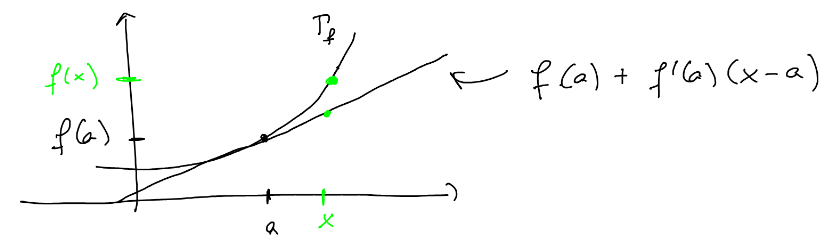
\includegraphics[width=0.7\linewidth]{figures/ableitung_erinnerung}
        \label{fig:ableitung_erinnerung}
    \end{figure}
    Für Abbildungen \( f\maps \reals^n\to \reals^n \) kann man analog definieren:
\end{erinnerung*}
\begin{definition}\index{Ableitung}
    Die \emph{Ableitung} einer Funktion \( f\maps U\to \reals^m \), \( U\subset \reals^n \) offen, an der Stelle \( a\in U \), ist, wenn sie existiert, eine Matrix \( \totalderivative{f}(a)\in \Mat(m\times n) \), die eine lineare Approximation von \( f \) ergibt:
    \begin{align*}
        f(x)=f(a)+\totalderivative{f}(a)\explain{\text{Matrix-Multiplikation}}{\matrixmult}(x-a)+R_a(x)\tag{\(*\)}\label{eq:ableitung:definition}
    \end{align*}
    Sie existiert genau dann, wenn
    \begin{align*}
        \overset{\underset{\downarrow}{\text{in }\reals^m}}{\lim_{x\explain{\text{in }\reals^n}{\goesto} a}}\frac{R_a(x)}{\explain[big]{\text{eine Norm in \( \reals^n \)}}{\norm{x-a}}}=0
    \end{align*}
    und ist in diesem Fall eindeutig durch \eqref{eq:ableitung:definition} bestimmt und man sagt, \( f \) ist \emph{differenzierbar}.
\end{definition}
\begin{bemerkungen*}
    \begin{enumerate}
        \item Für \( n=m=1 \) stimmt die Definition mit der Üblichen überein, da \( \frac{R_a(x)}{x-a}\goesto 0 \) \tiff \( \frac{R_a(x)}{\abs{x-a}}\goesto 0 \).
        \item Eindeutigkeit: Sei \( A \) \sd
        \begin{align*}
            f(x)\begin{aligned}[t]
                &=f(a)+A\matrixmult(x-a)+\tilde{R}_a(x)\\
                &=f(a)+\totalderivative{f}(a)\matrixmult (x-a)+R_a(x)
            \end{aligned}            
        \end{align*}
        Dann folgt:
        \begin{align*}
            \lim_{x \goesto a}(\underbrace{(A-\totalderivative{f}(a))\matrixmult (x-a)\cdot\quot{1}{\norm{x-a}}}_{=\frac{1}{\norm{x-a}}(R_a(x)-\tilde{R}_a(x))})=0.
        \end{align*}
        \timplies \( A-\totalderivative{f}(a)=0 \) (Nullmatrix), da wegen der Stetigkeit linearer Abbildungen \( \reals^n\to \reals^m \) der Grenzwert gleich \( (A-\totalderivative{f}(a))\matrixmult \lim \quot{(x-a)}{\norm{x-a}} \) ist und \( \norm{\lim \quot{(x-a)}{\norm{x-a}}}=1\neq 0 \).
        \item Wie in der \diffcourse{1} ist es oft zweckmäßig \( f \) an der Stelle \( a+h \) mit \( f \) an der Stelle \( a \) zu vergleichen (\( x=a+h \)).
        \begin{align*}
            f(a+h)=f(a)+\totalderivative{f}(a)\matrixmult h+\underline{R}_h(a)
        \end{align*}
        mit \( \lim_{h \goesto 0}\quot{(\underline{R}_h(x))}{\norm{h}}=0 \).
    \end{enumerate}
\end{bemerkungen*}
\begin{beispiele*}
    \begin{enumerate}
        \item \( f\maps \reals^n\to \reals^m \), \( f(x)=A\matrixmult x+b \), \( A\in \Mat(m\times n, \reals) \), \( b\in \reals^m \).
        \begin{align*}
            f(a+h)=f(a)+A\matrixmult h\implies \totalderivative{f}(a)=A.
        \end{align*}
        Insbesondere verschwindet die Ableitung einer konstanten Funktion.
    \item \( f\maps \reals^n \to \reals\), \( f(x)=\scalarproduct{x}{B\matrixmult x} \), \( \scalarproduct{\cdot}{\cdot} \) euklidisches Skalarprodukt, \( B\in \Mat(n\times n, \reals) \).
    \begin{align*}
        f(a+h)\begin{aligned}[t]
            &=\scalarproduct{a+h}{B\matrixmult (a+h)}\\
            &=\scalarproduct{a}{B\matrixmult a}+\scalarproduct{h}{B\matrixmult a}+\scalarproduct{a}{B\matrixmult h}+\scalarproduct{h}{B\matrixmult h}\\
            &\explain{\text{CHECK!}}{=}\scalarproduct{a}{B\matrixmult a}+\scalarproduct{(B+B^T)\matrixmult a}{h}+\scalarproduct{h}{Bh}. 
        \end{aligned}                
    \end{align*}
    Wegen (wähle \( \norm{\cdot}=\norm{\cdot}_{\text{E}} \))
    \begin{align*}
        \frac{\scalarproduct{a}{Bh}}{\norm{h}}\underset{\text{C-S}}{\leq}\frac{\norm{h}\cdot\norm{Bh}}{\norm{h}}\leq \norm{B}_{\text{op}}\cdot\norm{h}\goesto 0  \text{ für }h\goesto 0
    \end{align*}
    folgt: \( f \) ist in allen \( a\in \reals^n \) differenzierbar und
    \begin{align*}
        &\totalderivative{f}(a)\matrixmult h=\scalarproduct{(B+B^T)\matrixmult a}{h}=(b_1,\dots,b_n)\begin{pNiceMatrix} h_1 \\ \vdots \\ h_n \end{pNiceMatrix}\\
        \implies &\totalderivative{f}(a)=b=((B+B^T)\matrixmult a)^T\in \Mat(1\times n,\reals)\quad \forall h\in \reals^n. 
    \end{align*}
    \end{enumerate}
\end{beispiele*}
Aus der Definition folgt sofort
\begin{satz}
    Sei \( f\maps U\to \reals^m \), \( U\subset \reals^n \) offen, in \( a\in U \) differenzierbar. Dann ist \( f \) in \( a \) stetig.
\end{satz}
\begin{proof}
    \begin{align*}
        \lim_{h \goesto 0}f(a+h)\begin{aligned}[t]
            &=\lim_{h \goesto 0}(f(a)+\totalderivative{f}(a)+\underline{R}_a(h))\\
            &=f(a)+\explain[Big]{\explain{\text{Norm in \( \reals^m \)}}{\norm{\totalderivative{f}(a)\matrixmult h}}\leq \norm{\totalderivative{f}(a)}_{\text{op}}\cdot\explain{\text{Norm in \( \reals^n \)}}{\norm{h}}}{0}+\explain{\phantom{\text{Es gilt sogar meeehr!}}\text{Es gilt sogar \(\quot{\underline{R}_a(h)}{\norm{h}}\goesto 0\)}}{0}
        \end{aligned}
    \end{align*}
\end{proof}
\begin{satz}[Kettenregel]\index{Kettenregel}
    Seien \( U\subset \reals^n \), \( V\subset \reals^m \) offen, \( g\maps U\to \reals^m \), \( f\maps V\to \reals^k \), \( g(U)\subset V \). Ist \( g \) in \( a\in U \) differenzierbar und \( f \) in \( b=g(a) \), so ist die Verkettung \( f\circ g\maps U\to \reals^k \) in \( a \) differenzierbar und es gilt
    \begin{align*}
        \totalderivative+{f\circ g}(a)=\explain{\in \Mat(k\times m,\reals)}{\underbrace{\totalderivative{f}(g(a))}}\explain[big]{\in \Mat(m\times n),\reals}{\underbrace{\totalderivative{g}(a)}}.
    \end{align*}
\end{satz}
\begin{proof}
    \begin{align*}
        g(a+u)&=g(a)+A\cdot u+\underline{R}_a^g(u)\quad A=\totalderivative{g}(a)\tag{1}\label{eq:ableitung:kettenregel:g}\\
        f(b+v)&=f(b)+B\cdot v+\underline{R}_b^f(v)\quad B=\totalderivative{f}(b)\tag{2}\label{eq:ableitung:kettenregel:f}
    \end{align*}
    Setze speziell \( v\definedas g(a+u)-g(a)\overset{\eqref{eq:ableitung:kettenregel:g}}=A\cdot u+\underline{R}_a^g(u) \).
    \begin{align*}
        \implies f\circ g(a+u)\begin{aligned}[t]
            &=f(g(a+u))=f(g(a)+v)\eqstep{\text{Def } v}\\
            &\underset{\eqref{eq:ableitung:kettenregel:f}}{=}f(g(a))+B\matrixmult v+\underline{R}_b^f(v)\eqstep[p,v]{b=g(a)}\\
            &\explain{\text{Def \( v \) und \eqref{eq:ableitung:kettenregel:g}}}{=}f(g(a))+B\matrixmult A\matrixmult u+\explain{\text{zu zeigen: }\frac{\cdot}{\norm{u}}\goesto 0 \text{ für }u\goesto 0}{\underbrace{B\cdot\underline{R}_a^g(u)+\underline{R}_b^f(A\cdot u+\underline{R}_a^g(u))}}.
        \end{aligned}        
    \end{align*}
    \begin{itemize}
        \item \(\frac{\underline{R}_a^g(u)}{\norm{u}}\goesto 0 \) \timplies \texists \( C>0 \) \sd \( \norm{\underline{R}_a^g(n)}\leq C\norm{n} \).
        \item \( \frac{\underline{R}_b^f(v)}{\norm{v}}\goesto 0 \) \timplies \texists \( \underline{r}_b^f \) \sd \( \underline{R}_b^f(v)=\norm{v}\underline{r}_b^f(v) \)mit \( \underline{r}_b^f(v)\goesto 0 \) (\( v\goesto 0 \)).
    \end{itemize}
    \begin{align*}
        \implies &\explain{\text{Norm in \( \reals^k \)}}{\underline{R}_b^f(A\matrixmult u +\underline{R}_a^g(u))}\leq \explain{\text{Norm in \( \reals^k \)}}{\overbrace{A\matrixmult u +\underline{R}_a^g(u)}^{\leq\p*{ \norm{A}_{\text{op}}+C }\norm{u}}}\cdot\norm{\underline{r}_b^f(\underbrace{Au+\underline{R}_a^g(u)}_{\mathclap{\goesto 0 \text{ für }u\goesto 0}})}\\
        \implies &\frac{\underline{R}_b^f(A\matrixmult u+\underline{R}_a^g(u))}{\norm{u}}\goesto 0\quad (u\goesto 0).
    \end{align*}
\end{proof}
\begin{satz}[Produktregel, Quotientenregel]\index{Produktregel}\index{Quotientenregel}
    Seien \( f,g\maps U\to \reals \), \( U\subset \reals^n \) offen, differenzierbar in \( a\in U \). Dann gilt
    \begin{enumerate}
        \item \label{produktregel} \( f\cdot g \) ist differenzierbar in \( a \) und es gilt
        \begin{align*}
            \totalderivative+{f\cdot g}(a)=\totalderivative{f}(a)\matrixmult g(a)+f(a)\matrixmult \totalderivative{g}(a).
        \end{align*}
        \item \label{quotientenregel} Ist \( g(a)\neq 0 \) so gilt: \( \quot{f}{g} \) ist auf einer Umgebung von \( a \) definiert und differenzierbar in \( a \) und es gilt 
        \begin{align*}
            \totalderivative+{\quot{f}{g}}(a)=\totalderivative{f}(a)\cdot\frac{1}{g(a)}-f(a)\cdot\frac{1}{g(a)^2}\cdot \totalderivative{g}(a).
        \end{align*}
    \end{enumerate}
    
\end{satz}
\begin{proof}
    \begin{proofdescription}
        \item[\ref{produktregel}]
        \begin{align*}
            f(a+h)&=f(a)+\totalderivative{f}(a)\matrixmult h+\underline{R}_{a}^f(h)\\
            g(a+h)&=g(a)+\totalderivative{g}(a)\matrixmult h+\underline{R}_{a}^g(h)\\
            f\cdot g(a+h)&\begin{aligned}[t]
                &=\p*{ f(a)+\totalderivative{f}(a)\matrixmult h+\underline{R}_{a}^f(h) }\p*{ g(a)+\totalderivative{g}(a)\matrixmult h+\underline{R}_{a}^g(h) }\\
                &=\begin{aligned}[t]
                    &f(a)\cdot g(a)+(\underbrace{\totalderivative{f}(a)\matrixmult g(a)}_{\in \Mat(1\times n,\reals)})\matrixmult h+(\underbrace{f(a)\matrixmult \totalderivative{g}(a)}_{\in \Mat(1\times n,\reals)})\matrixmult h\\
                    &+\underbrace{(\totalderivative{f}(a)\matrixmult h+\underline{R}_a^f(h))(\totalderivative{g}(a)\matrixmult h+\underline{R}_a^g(h))}_{\frac{\cdot}{\norm{h}}\goesto 0 \text{ für }h\goesto 0}.
                \end{aligned}
            \end{aligned}            
        \end{align*}
        \item[\ref{quotientenregel}] \( g \) ist in \( a \) stetig \timplies \texists Umgebung von \( a \) \sd \( g(x)\neq 0 \) \tforall \( x\in U \) (wie in der \diffcourse{1}: Sei \obda \( g(a)>0 \). Sei \( \varepsilon\definedas \quot{g(a)}{2} \). Sei \( \norm{\cdot} \) irgendeine Norm auf \( \reals^n \). Dann gibt es ein \( \delta>0 \) \sd
        \begin{align*}
            &\abs{g(x)-g(a)}<\varepsilon\quad \forall x\in B_{\delta}^{\norm{\cdot}}(a)\\
            \implies &-\frac{g(a)}{2}<g(x)-g(a)<\frac{g(a)}{2}\quad \forall x\in B_{\delta}^{\norm{\cdot}}(a),
        \end{align*}
        also \( 0<\frac{g(a)}{2}<g(x)<\frac{3}{2}\frac{g(a)}{2} \).) \timplies Auf \( U \) ist \( \quot{f}{g} \) wohldefiniert. Die Berechnung der Ableitung ist analog zu \ref{produktregel}, nachdem man sich überlegt hat, dass
        \begin{align*}
            \frac{1}{g}=\text{Inv}\circ g,\quad \text{Inv}(t)=\frac{1}{t}
        \end{align*}
        und somit nach der Kettenregel
        \begin{align*}
            \totalderivative+*{\frac{1}{g}}(a)=\totalderivative{\text{Inv}(g(a))}\cdot \totalderivative{g}(a)
        \end{align*}
        und \( D \text{Inv}(t)=-\frac{1}{t^2} \) (\diffcourse{1}).
    \end{proofdescription}    
\end{proof}
\section{Geometrische Anschauung, partielle Ableitung}
\diffcourse{1}: Ableitung beschreibt Rate der Veränderung. Höher-dimensional: Sei \( f\maps U\to \reals \), \( U\subset \reals^n \). Betrachte den Graph \( \Gamma_f=\Set{(x,f(x))|x\in U} \) (\vgl die Diskussion bei \ref{stetigkeit:beispiel:gebrochen_rationale_funktionen})
\begin{figure}[H]
    \centering
    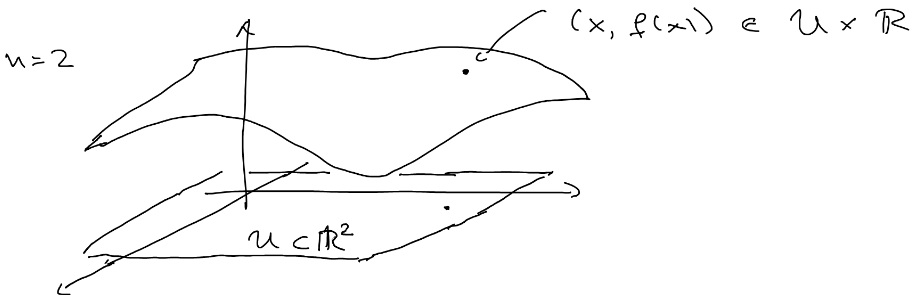
\includegraphics[width=0.8\linewidth]{figures/r2_zu_r_funktion_veranschaulichung}
    \label{fig:r2_zu_r_funktion_veranschaulichung}
\end{figure}
\begin{definition*}[Niveau-Mengen]\index{Niveau-Menge}
    Zu \( c\in \reals \) setze \( N_f(c)\definedas \Set{x\in U|f(x)=c} \).
\end{definition*}
\begin{beispiel*}
    \begin{figure}[H]
        \centering
        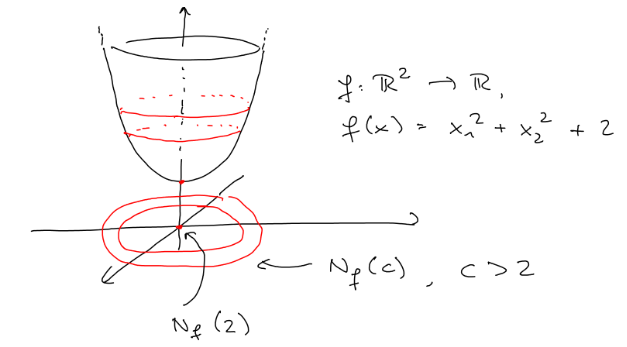
\includegraphics[width=0.5\linewidth]{figures/niveau_menge_beispiel}
        \caption*{Es gilt \( N_f(c)=\emptyset \) für \( c<2 \).}
        \label{fig:niveau_menge_beispiel}
    \end{figure}
    Entlang der Niveauflächen ist \( f \) konstant. Wie wird das in der Ableitung sichtbar?

    Im Beispiel oben ist \( \totalderivative{f}(a)=(2a_1,2a_2) \) (check!). Sei \( a=(r\Cos{\phi}, r\Sin{\phi}) \), \( r>0 \). Betrachte \( f(a+h)=f(a)+\totalderivative{f}(a)\matrixmult h+\underline{R}_a(h) \). Ist \( h=\textcolor{Blue}{(-\varepsilon \Sin{\phi}, \varepsilon \Cos{\phi})} \), \( \varepsilon>0 \) (in \enquote{Richtung} der Niveaumenge), so ist \( \totalderivative{f}(a)\matrixmult h=0 \).
    \begin{figure}[H]
        \centering
        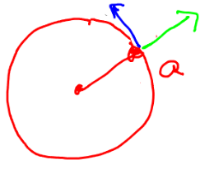
\includegraphics[width=0.2\linewidth]{figures/in_richtung_und_orthogonal_der_niveaumenge}
        \label{fig:in_richtung_und_orthogonal_der_niveaumenge}
    \end{figure}
    Ist dagegen \( h=\textcolor{Green}{(\varepsilon \Cos{\phi}, \varepsilon \Sin{\phi})} \) (von der Niveaumenge weg), so ist \( \totalderivative{f}(a)\matrixmult h=2r\varepsilon>0 \). Das wollen wir im Folgenden systematisch studieren.
\end{beispiel*}
\begin{definition*}\index{Richtungsableitung}
    Sei \( f\maps U\to \reals^m \), \( U\subset \reals^n \) offen, gegeben. Für \( a\in U \) und \( v\in \reals^n \) heißt der Grenzwert (falls er existiert)
    \begin{align*}
        \partial_v f(a)\definedas \explain{\text{in \( \reals^m \)}}{\lim_{t \goesto 0}}\frac{f(a+tv)-f(a)}{t}
    \end{align*}
    die \emph{Richtungsableitung von \( f \)} in \( a \) in Richtung \( v \).
    \begin{figure}[H]
        \centering
        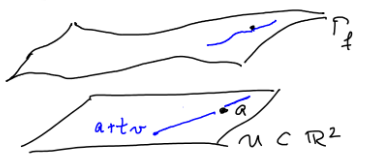
\includegraphics[width=0.5\linewidth]{figures/richtungsableitung}
        \label{fig:richtungsableitung}
    \end{figure}
\end{definition*}
\begin{bembspe}
    \begin{enumerate}
        \item \( \partial_v f(a)=\evaluateat{\frac{d}{dt}}{t=0} g_{a,v}(t)=g_{a,v}'(0) \), \( g_{a,v}(t)=f(a+tv) \).
        \item \( f=(f_1,\dotsc,f_m)^T \), so gilt
        \begin{align*}
            \partial_v f(a)=(\partial_v f_1(a),\dotsc, \partial_v f_m(a))^T
        \end{align*}
            \item \( f\maps (x_1,x_2)\mapsto x_1^2+x_2^2+2 \). Sei \( a=(r\Cos{\phi}, r\Sin{\phi}) \). Ist \( v=(\varepsilon \Cos{\phi}, \varepsilon\Sin{\phi}) \), so ist
            \item \begin{align*}
                g_{a,v}(t)=((r+\varepsilon t)\Cos{\phi})^2+((r+\varepsilon t)\Sin{\phi})^2+2
            \end{align*}
            und somit \( \partial_v f(a)=g_{a,v}'(0)=2(r+\varepsilon \cdot 0)\varepsilon=2r\varepsilon \).
            
            Ist \( v=(-\varepsilon \Sin{\phi}, \varepsilon \Cos{\phi}) \), so ist
            \begin{align*}
                g_{a,v}(t)=(r \Cos{\phi}-\varepsilon t\Sin{\phi})^2+(r\Sin{\phi}+\varepsilon t \Cos{\phi})^2
            \end{align*}
            und somit
            \begin{align*}
                \partial_v f(a)=g_{a,v}'(0)=2(r\Cos{\phi}-0)(-\varepsilon \Sin{\phi})+2(r\Sin{\phi}+0)(\varepsilon \Cos{\phi})=0.
            \end{align*}
            Das ist kein Zufall, denn es gilt
    \end{enumerate}
\end{bembspe}
\begin{satz}
    Sei \( f\maps U\to \reals^m \), \( U\subset \reals^n \) offen, in \( a\in U \) differenzierbar. Dann besitzt \( f \) die Richtungsableitungen
    \begin{align*}
        \partial_v f(a)=\totalderivative{f}(a)\matrixmult v\quad \forall v\in \reals^n
    \end{align*}
    und \( \totalderivative{f}(a) \) hat bezüglich der Standardbasis \( e_1,\dotsc, e_n \) die Matrix Darstellung
    \begin{align*}
        \begin{pNiceMatrix} \partial_1 f & \Cdots  & \partial_n f \end{pNiceMatrix}=\begin{pNiceMatrix}
            \partial_1 f_1(a) & \Cdots & \partial_n f_1(a) \\
            \partial_1 f_2(a) & \Cdots & \partial_n f_2(a)  \\
            \Vdots &  & \Vdots\\
            \partial_1 f_m(a) & \Cdots & \partial_n f_m(a) 
        \end{pNiceMatrix}\in \Mat(m\times n,\reals),
    \end{align*}
    \enquote{Jacobi-Matrix}, wobei \( \partial_j f(a)=\partial_{e_j}f(a)=\totalderivative{f}(a)\matrixmult e_j=j \)-te Spalte.
\end{satz}
\begin{proof}
    Für \( v=0 \) sind beide Seiten \( 0 \) \checkmark.

    Für \( v\neq 0 \) betrachte
    \begin{align*}
        \begin{aligned}[t]
            &\rphantom{=}\norm{\quot{(f(a+tv)-f(a))}{t}-\totalderivative{f}(a)\matrixmult v}_{\sim\ (\text{Norm auf \( \reals^m \)})}\\
            &=\frac{1}{\abs{t}}\norm{f(a+tv)-(f(a)+\totalderivative{f}(a)\matrixmult(tv))}_{\sim}\\
            &\explain{\text{Homogenität }\norm{\cdot}}{=}\frac{1}{\explain{\text{Norm auf \( \reals^n \)}}{\norm{t\cdot v}}}\norm{f(a+tv)-(f(a)+\totalderivative{f}(a)\matrixmult(tv))}_{\sim}\cdot\norm{v}.
        \end{aligned}
    \end{align*}
    Differenzierbarkeit \timplies strebt gegen \( 0 \) für \( tv\goesto 0 \), also für \( t\goesto 0 \) \timplies Die Richtungsableitungen existieren und 
    \begin{align*}
        \partial_v f(a)=\totalderivative{f}(a)\matrixmult v
    \end{align*}
    und bezüglich der kanonischen Basen gilt
    \begin{align*}
        \equalto{\begin{pNiceMatrix} \partial_j f_1(a) \\ \Vdots \\ \partial_j f_m(a) \end{pNiceMatrix}}{\partial_j f(a)}=\totalderivative{f}(a)\matrixmult e_k=j \text{-te Spalte von \( \totalderivative{f}(a) \)}.
    \end{align*}
\end{proof}
\begin{achtung*}
    Umgekehrt genügt die Existenz der Richtungsableitungen \( \partial_1 f,\dotsc, \partial_n f \) nicht, um Differenzierbarkeit zu garantieren!
    \begin{beispiel*}
        \begin{align*}
            f(x,y)=\begin{cases}
                \frac{xy}{x^2+y^2}&(x,y)\neq (0,0)\\
                0 &(x,y)=(0,0)
            \end{cases}
        \end{align*}
    \end{beispiel*}
    \( \partial_1 f(x,y)=\evaluateat{\frac{d}{dt}}{t=0}f(x+t,y) \), \( \partial_2 f(x,y)=\evaluateat{\frac{d}{dt}}{t=0} f(x,y+t) \). Wegen \( f(x,0)=0 \quad \forall x \), \( f(0,y)=0\quad \forall y \), ist \( \partial_1 f(0,0)=0=\partial_2 f(0,0) \). Aber \( f  \) ist in \( 0 \) nicht stetig (betrachte etwa \( (\quot{1}{n},\quot{1}{n}) \)), also nicht differenzierbar.
\end{achtung*}




